\documentclass[twoside,11pt]{article}

% Any additional packages needed should be included after jmlr2e.
% Note that jmlr2e.sty includes epsfig, amssymb, natbib and graphicx,
% and defines many common macros, such as 'proof' and 'example'.
%
% It also sets the bibliographystyle to plainnat; for more information on
% natbib citation styles, see the natbib documentation, a copy of which
% is archived at http://www.jmlr.org/format/natbib.pdf

\usepackage{jmlr2e}
%\usepackage{parskip}

% Definitions of handy macros can go here
\newcommand{\dataset}{{\cal D}}
\newcommand{\fracpartial}[2]{\frac{\partial #1}{\partial  #2}}
% Heading arguments are {volume}{year}{pages}{submitted}{published}{author-full-names}

% Short headings should be running head and authors last names
\ShortHeadings{95-845: MLHC Final Project}{LI}
\firstpageno{1}

\begin{document}

\title{Heinz 95-845: Forecasting Postoperative Mortality after General Surgery Based on MIMIC III Data on \\Machine Learning for Health Care}

\author{\name Xinmi Li \email xinmil@andrew.cmu.edu \\
       \addr Heinz College\\
       Carnegie Mellon University\\
       Pittsburgh, PA, United States
       } 

\maketitle

\begin{abstract}
  This paper aims to use machine learning models to predict postoperative mortality for patients in intensive care units (ICU) after general surgery. Multiple machine learning algorithms are trained and tested with the data collected in Multiparameter Intelligent Monitoring in Intensive Care III (MIMIC III) database. Through these models, items considered to be significant in post-surgery care are examined and their contribution to post-surgery death are disccussed in this paper. In this paper, the performance of each algorithm is also compared with each other, to suggest on the most useful and reliable model that could be used in future postoperative mortality prediction.
\end{abstract}

\section{Introduction}
In medical field, the traditional method to analyzing the effect of an intervention is to conduct a randomized clinical trial and analyze the outcomes. Though high levels of recommendation could derive from them, with many limitations such as the size of population involved in the trial and ethical concerns, randomized clinical trials may not be able to be launched or completed, or the conclusions could be not broadly applicable. Besides, the complicated recruiting stage, the compliance issue of participants, and the long period of the trial and follow-ups make the randomized clinical trial unefficient and costly.

Recent advances in machine learning and the transfer from paper health records to eletronic health records have provided huge opportunities to health care research. With large volume of patient data and the high-speed data processing, we are now able to research on the topics that are used to be impposible for randomized clinical trial. 

MIMIC III database is a large and freely available database that consists of deidentified health-related data on over 40,000 patients collected from ICU of the Beth Israel Deaconess Medical Center between 2001 and 2012 \citet{cite1}. Some amount of progress on mortality prediction has been made by studying MIMIC III data. One research uses the abundance of ICU data to analyze the relationship between using selective serotonin reuptake inhibitors and the increase of mortality \citep{cite2}, but it only does statistical tests on the outcome instead of building machine learning models. And another reaserch makes mortality predictions among patients with sepsis and hypotension by using dynamic data during hypotensive episode\citep{cite3}. Although it only uses logistic regression to build the model, it has the movelty that using multiple perform measures to compare this model with traditional medical protocols. And another study builds a targeted real-time early warning score for septic shock by using lab data \citep{cite4}, which outperforms other widely-used protocols.

In this work, we use the MIMIC III data to predict the post-surgery mortality for ICU patients who just had genral surgery. Unlike to other studies using MIMIC data, this work makes the prediction not related to a specific condition. The purpose of it is to have a more general forecast that can be applied to all ICU patients with general surgery, and to provide a guide for nurses to provide better post-surgery care through the examination of indicators of mortality.

In Section 2, we provide background on the postoperative mortality. In section 3, we have a basic elaboration of the models used in this study. Then in section 4, experimental setup is provided to allow for replication of the study. Section 5 gives the results of the model. And more discussions on this study and related work are in section 6.

\section{Background} \label{background}
With more and more emphases on heath care quality and patient safety, lowering the postoperative risk is extremely significant. Although the national death rate from complications of medical and surgical care is decreasing over years \citet{cite5}, post-surgery death is still a big issue especially for the acute or unplanned surgery. Therefore, good postoperative care is important. To have a guidance on indicators of postoperative risk of death means not only better patient safety outcomes but also a relief from alert fatigue for nurses.

\begin{figure}[htbp]
  \centering 
  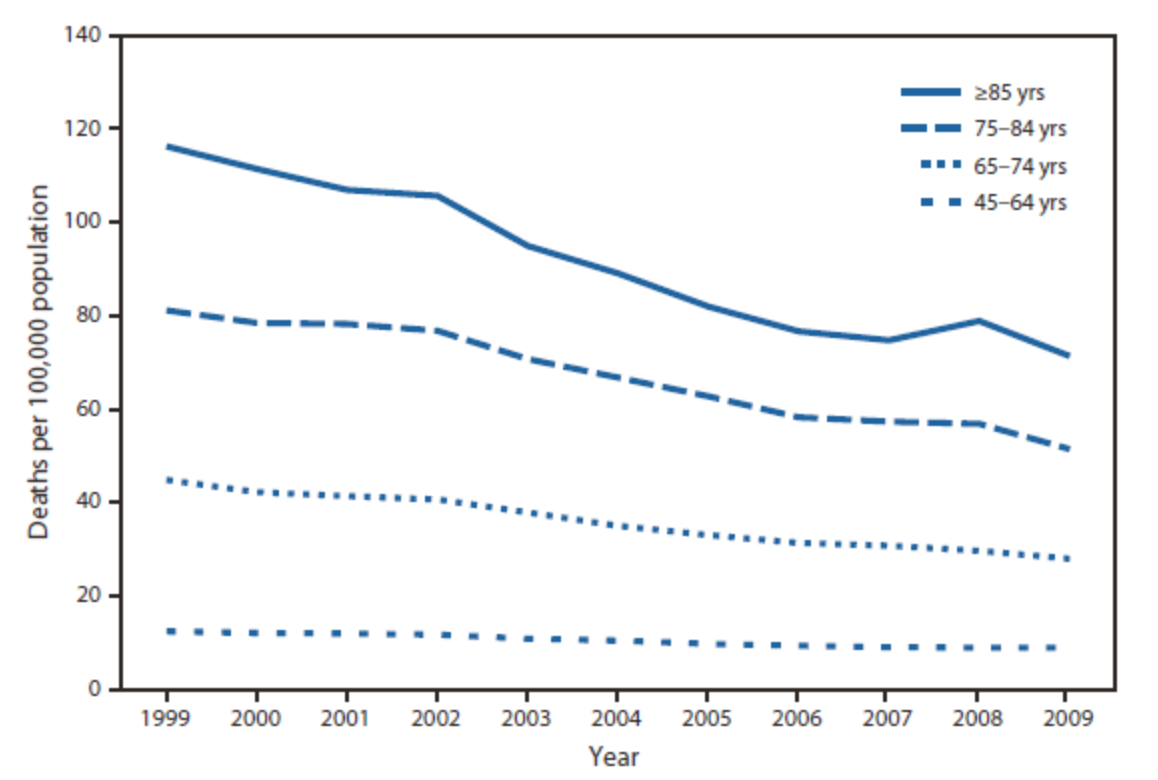
\includegraphics[height=10cm, width=15cm]{fig1} 
  \caption{Death Rate From Complications of Medical and Surgical Care Among Adults Aged ≥45 Years, by Age Group — United States, 1999~2009}
  \label{fig1} 
\end{figure} 

\section{Your Model Name Here} \label{model}
This section describes your model and references the notation you introduced in the Background Section. \textbf{Figures are definitely helpful here}, so that someone who is in your area can visualize how your approach is novel, and someone who is not in your area can visualize what you are doing.

If you introduce new mathematical or statistical methods, use the terminology you defined in Section \ref{background} and define your model. Give the technical details and remember: do be precise and do be concise.

If you are combining existing methods, then you don't need to provide a ton of detail: feel free to just cite other packages and papers and tell us how you put them together.  

If you developed new code that does not (should not) contain sensitive or private information, include a reference, e.g.:

`` Code is available at \url{http://my.github.page.com} ''

\section{Experimental Setup} \label{experiment}
\emph{Note: if the paper is more about the application than the method, this Section may be entitled Methods and appear before Section \ref{model}}

By reading the Experimental Setup, your reader should have the information necessary to replicate the study.

Describe the cohort/data. Provide information about the population, the inclusion and exclusion criteria, what data were extracted, how features were processed, etc. In fact, you may want the following headings. \textbf{A flow chart can be very helpful} to illustrate the experimental setup, study design, inclusion/exclusion process, etc.

For more clinical application papers, each of the sections above might be several paragraphs or pages because we really want to understand the setting.

\subsection{Cohort Selection} 
Describe how the samples you used were selected to form your cohort and also to provide cohort descriptive statistics. In methodologic papers, the ``Table 1'' describing the population by covariate summary statistics goes here. In application papers, ``Table 1'' leads the Results Section. Relevant information about the study design, such how cases and controls were identified, goes here. See Section \ref{results} for an example of how to build a table in LaTeX.

\subsection{Data Extraction} 
Describe the pipeline from raw data to processed data. Figures can be helpful. What assumptions did you make? How did you deal with missing data? Do not place interpretations here except possibly for short justification phrases. Longer discussions about the assumption you made go in the Discussion Section.

\subsection{Feature Choices} 
What features were used? What conversions were necessary? What assumptions (e.g. i.i.d.) are made? with how you might have converted the raw data into features that were used in your algorithm. 

\subsection{Comparison Methods}
To evaluate your model, often times you will compare against existing models.
If so, include them here with a brief description, citation, and any tweaks you made for your experiment.

\subsection{Evaluation Criteria}
Evaluation methods belong here as well.
Perhaps you used accuracy and the AUROC--explain why these are most useful measures of the outcome.

\section{Results} \label{results}

Present the results here.
Do not describe how the results were obtained.
Those descriptions belong in Section \ref{experiment}.

Typically there are multiple parts and subparts of your study.
Use subsections to report the results.

\subsection{Results on Application A} 

Give us some numbers about how well your method works, especially in comparison to some baselines.
You should provide a summary of the results in the text, as well as in tables (such as table~\ref{tab:example}) and figures (such as figure~\ref{fig:example}).  

You may use subfigures/wrapfigures (LaTeX packages) so that figures don't have to span the whole page or multiple figures are side by side.

\begin{table}[htbp]
  \centering 
  \begin{tabular}{lclc} 
    Method & Outcome (\%) \\ 
    \hline \\[-11pt]
    Us & 20.1 \\ 
    Baseline & 18.2 \\ \hline 
  \end{tabular}
  \label{tab:example} 
    \caption{Outcome by method used. These are our results.} 
\end{table}

\begin{figure}[htbp]
  \centering 
  
\includegraphics[width=1.5in]{smile.jpeg} 
  \caption{Example smile graphic.}
  \label{fig:example} 
\end{figure} 

\subsection{Results on Application B} 

Did more than one experiment type?

\section{Discussion and Related Work} 

This is where you characterize the outcomes of your method and draw conclusions from you experiment.
The discussion will build upon the Introduction and the Results sections to synthesize where your contribution brings the field. Discuss any implications of your work. 
Discuss limitations of your work.
Are there situations where you should and should not use your method.
What implications are there on policy making, clinical decision making, or future research activities?
Remember to contextualize your work with respect to related work and provide references.

\section{Conclusion} 
Summarize your work one more time, this time assuming the reader has read your paper.
Build suspense for what your next extension to this method would be.

% ACKNOWLEDGEMENTS ONLY GO IN THE CAMERA-READY, NOT THE SUBMISSION
% \acks{Many thanks to all collaborators and funders!}

\bibliography{citation}

\appendix
\section*{Appendix A.}
Some more details about those methods, so we can actually reproduce them.

\end{document}
